\documentclass[11pt,ngerman,a4paper]{article}
%Gummi|061|=)
\usepackage{amsmath}
\usepackage{a4wide}
\usepackage{url}
\usepackage{amsthm}
\usepackage{amsbsy}
\usepackage{amssymb}
\usepackage[utf8]{inputenc}
\usepackage{rotating} 
\usepackage{here}
\usepackage{graphicx}
\usepackage{paralist}
\usepackage{selinput}
\usepackage[separate-uncertainty=true]{siunitx}
\usepackage{booktabs}
\sisetup{}
\SelectInputMappings{%
adieresis={ä},
germandbls={ß},
}
\title{\textbf{Versuch V504: Thermische Elektronenemission}}
\author{Martin Bieker\\
		Julian Surmann\\
		\\
		Durchgef\"{u}hrt am 17.06.2014\\
		TU Dortmund}
\date{}
\usepackage{graphicx}
\begin{document}
\renewcommand\tablename{Tabelle}
\renewcommand\figurename{Abbildung}
\maketitle
\thispagestyle{empty}
\newpage
\clearpage
\setcounter{page}{1}


\section{Einleitung}
In diesem Versuch wird die sogenannte Thermische Elektronenemission untersucht, dabei handelt es sich um die Auslösung von Elektronen aus einer Metalloberfläche mit Hilfe von thermischer Energie. Die Temperaturabhängigkeit dieses Vorganges ist von besonderem Interesse.
\section{Theorie}
\section{Auswertung}
\subsection{Bestimmung des Sättigungsstroms}
Zur Bestimmung des temperaturabhängigen Sättigungsstroms der Diode wurde der Strom in Abhängigkeit vom der Spannung zwischen Anode und Kathode gemessen. Diese Daten befinden sich in Tabelle \ref{tab_a}. In Abbildung \ref{abb_a} werden die ermittelten Kennlinien graphisch dargestellt. 
\begin{figure}[htp]
\centering
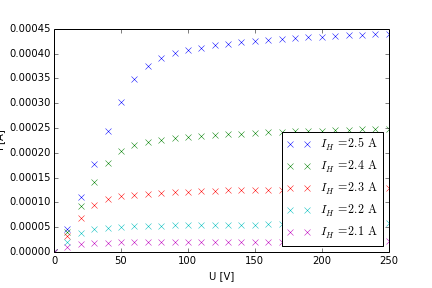
\includegraphics[scale=0.8]{plot_a.png}
\caption{Kennlinie der Hochvakuumdiode in Abhängigkeit von der Temperatur.}
\label{abb_a}
\end{figure}

\noindent
Es ist erkennbar, dass der Strom innerhalb des untersuchten Spannungsbereichs das jeweilige temperaturabhängige Sättigungsniveau erreicht. Somit entspricht der Sättigungsstrom näherungsweise dem höchsten gemessenen Wert von $I$ der jeweiligen Messreihe. Daher gilt:
\begin{itemize}
\item $I_1 = \SI{440}{\micro\ampere}$
\item $I_2 = \SI{248}{\micro\ampere}$
\item $I_3 = \SI{129}{\micro\ampere}$
\item $I_4 = \SI{58}{\micro\ampere}$
\item $I_5 = \SI{22}{\micro\ampere}$
\end{itemize}

\subsection{Verifizierung Langmuir-Schottkyschen Gesetztes}
In diesem Versuchsteil wird das Raumladungsgebiet der Kennlinie genauer untersucht.
Hier soll der Exponent $q$ der Strom-Spannungsbeziehung 
\[
I = k\cdot x^q
\]
bestimmt werden. Dazu sind in Abbildung \ref{plot_b} sind die Messpunkte für die maximale Heizleistung ($I_H = \SI{2.5}{\ampere}$) doppelt logarithmisch aufgetragen. In dieser Darstellung ist der lineare Zusammenhang
\[
\ln\left(\frac{I}{\si{\ampere}}\right) = q\cdot \ln\left(\frac{U}{\si{\volt}}\right)+ \ln\left(\frac{k}{\si{\ampere\per\volt}}\right)
\]
erkennbar. Durch eine lineare Ausgleichsrechnung ergibt sich:
\begin{itemize}
\item $q = \num{1.1317+-0.0011}$
\item $\ln\left(\frac{k}{\si{\ampere\per\volt}}\right) = \num{-12.531+-0.013}$ 
\end{itemize}
Die durch diese Werte bestimmte Ausgleichsgerade ist ebenfalls in Abbildung \ref{plot_b} dargestellt.
Die Abweichung von $q$ zum Langmuir-Schottkyschen Gesetz mit 
\[
q_{theo} = \frac32
\]
beträgt:
\[
\Delta q = \frac{|q_{theo}-q|}{q_{theo}} = \SI{24.55}{\percent}\rm.
\]
\subsection{Untersuchung des Anlaufstromgebiets}
\subsection{Bestimmung der Temperatur der Kathode}
\subsection{Berechnung der Austrittsarbeit des Kathodenmaterials}
\section{Diskussion}

\section{Quellen}
\begin{enumerate}[{[}1{]}]
\item Entnommen der Praktikumsanleitung \textit{} der TU Dortmund. \\
Download am 01.06.14 unter:\\
 \url{http://129.217.224.2/HOMEPAGE/PHYSIKER/BACHELOR/AP/SKRIPT/V703.pdf}
\end{enumerate}

\section{Anhang}
\begin{itemize}
\item Tabellen
\item Auszug aus dem Messheft
\end{itemize}
\end{document}
